\section{Zielsetzung}

Ziel dieses Versuches ist es, die Halbwertszeiten von $\ce{^51 V}$ und von $\ce{^134 Rh}$ zu bestimmen, indem stabile Kerne
mit Neutronen aktiviert werden.

\section{Theorie}
\label{sec:Theorie}
Atomkerne sind stabil und zerfallen nicht, wenn die Anzahl der Neutronen und Protonen in einem bestimmten 
Stabilitätsbereich liegt. Die meisten Atome sind stabil, wenn circa 20\,\% bis 50\,\% mehr Neutronen als Protonen den Kern bilden.
Eine besondere Kenngröße des Zerfalls ist die Halbwertszeit $T$, welche die Zeit beschreibt, in der von einer sehr großen Anzahl
an Kernen die Hälfte zerfallen ist.

\subsection{Aktivierung mit Neutronen}
Damit auch kleine Halbwertszeiten $T$ bestimmt werden können, lässt sich die Methode der Aktivierung von Atomkernen 
durch Neutronenbeschuss anwenden.
Dabei wird ein stabiler Kern mit langsamen Neutronen beschossen wodurch dieser angeregt wird. Der Kern in diesem Zustand 
wird als Zwischen- oder Compoundkern bezeichnet. Dieser angeregte Zwischenkern geht unter Emission eines Photons in einen Grundzustand
über. Der Zwischenkern befindet sich nach der Abgabe eines Photons nicht mehr in einem angeregten, jedoch in einem instabilen Zustand.
Durch einen $\beta^{-}$-Zerfall und somit der Abgabe eines Elektrons gelangt der Kern erneut in einen stabilen Zustand. Die ablaufenden 
Reaktionen folgen den Gleichungen
\begin{align*}
    \ce{^{\symup{m}}_{\symup{z}} A + ^{1}_0n \to ^{m{+1}}_{\symup{z}}{A^{*}} \to ^{m{+1}}_{\symup{z}}A} + \gamma\\
    \ce{^{m{+1}}_{\symup{z}}A \to ^{m{+1}}_{z{+1}}C }+ \beta ^{-} + E_{\text{kin}} + \overline{\nu}.
\end{align*}

Die Neutronen müssen eine langsame Geschwindigkeit aufweisen, da so die
Wahrscheinlichkeit, dass sie tatsächlich auf den Kern treffen größer ist. Dies hängt mit dem Wirkungsquerschnitt der Kerne
zusammen.

\subsection{Freisetzung langsamer Neutronen}
\label{sec:Neutronenaktivierung}
Die langsamen Neutronen werden durch eine Kernreaktion von $\ce{^226 Ra}$ und $\ce{^9 Be}$ freigesetzt. Dies geschieht, da
$\ce{^226 Ra}$ ein natürlicher $\alpha$-Strahler ist und so $\ce{^9 Be}$ mit einem Heliumkern gemäß
\begin{equation*}
    \ce{^9_4 Be} + \ce{^4_2 } \alpha \to \ce{^12_6 C} + \ce{^1_0 n}
\end{equation*}
reagiert.
Direkt nach der Freisetzung sind die Protonen sehr schnell, weshalb sie in Paraffin abgebremst werden. In \autoref{fig:Neutronenquelle}
ist ein schematischer Aufbau der in diesem Versuch verwendeten Neutronenquelle zu sehen.
\begin{figure}[H]
    \centering
    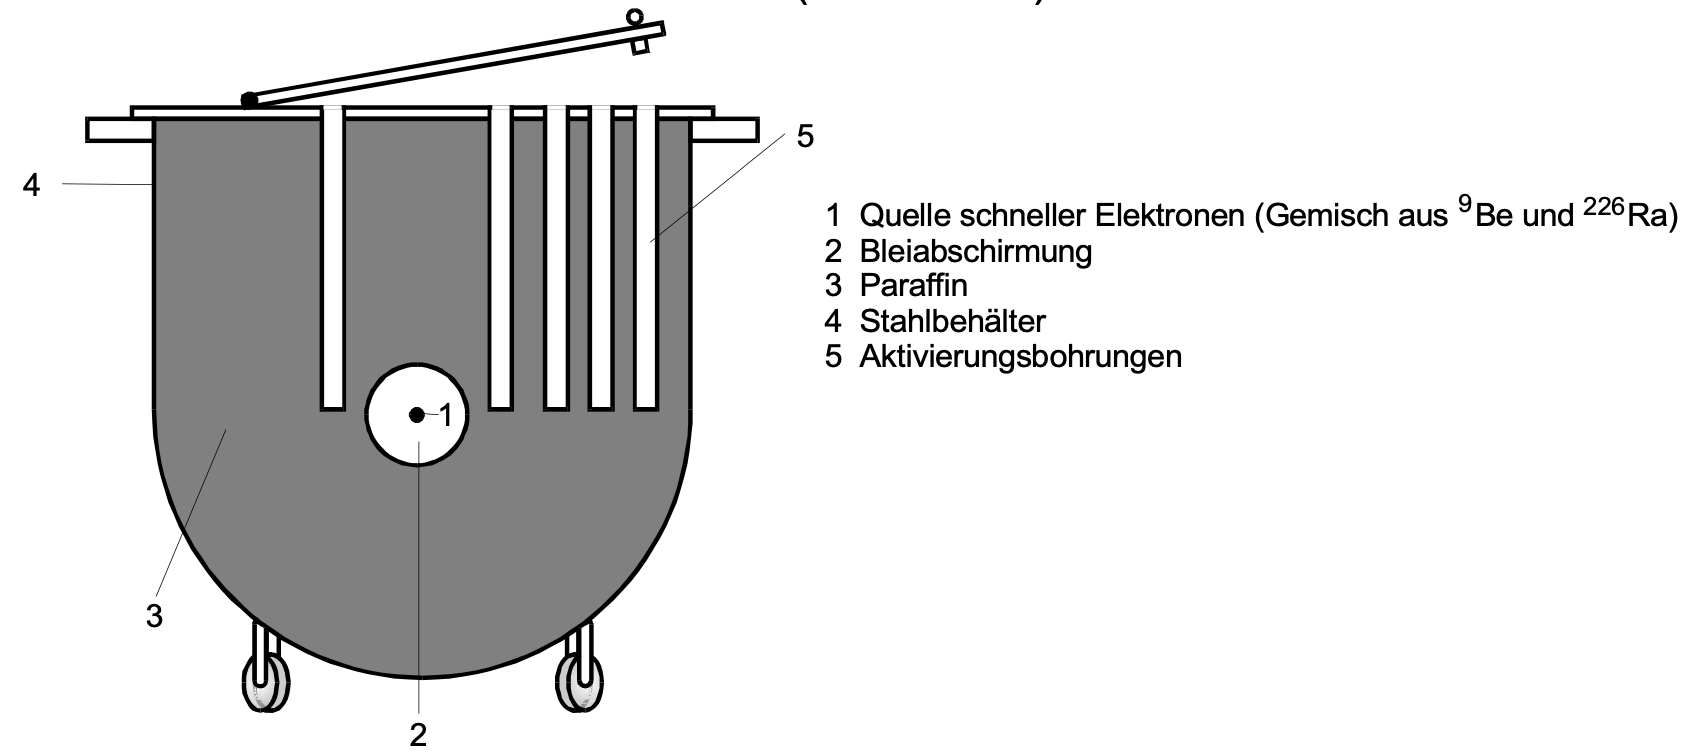
\includegraphics[height=5cm]{content/pics/Neutronenquelle.png}
    \caption{Aufbau der Neutronenquelle \cite{v702}.}
    \label{fig:Neutronenquelle}
\end{figure}

\subsection{Zerfall instabiler Isotope}
Die Anzahl der zerfallenen beziehungsweise nicht zerfallenen Kerne steht in einem exponetiellen Zusammenhang mit der Zeit.
Es gilt die Beziehung
\begin{equation}
    N(t)=N_0\symup{e}^{-\lambda t} \label{eq:Zerfall}
\end{equation}
wobei $N$ die Anzahl der nicht zerfallenen Kerne und $\lambda$ die Zerfallskonstante ist.

Die Halbwertszeit, also die Zeit, nachder die Hälfte der ursprünglichen Kerne zerfallen ist, ergibt sich direkt aus
Gleichung~\eqref{eq:Zerfall} zu
\begin{equation}
    T = \frac{\ln 2}{\lambda}. \label{eq:Halbwertszeit}
\end{equation}

Die Größe $N(t)$ wird in einem bestimmten Zeitintevall $\symup{\Delta}t$ gemessen, sodass das 
Zerfallsgesetz~\eqref{eq:Zerfall} geschrieben wird als
\begin{align*}
    N_{\symup{\Delta }t}(t) &= N(t) - N(t+\symup{\Delta} t) \\
    \ln(N_{\symup{\Delta }t}(t)) &= \ln(N_0)(1-\symup{e}^{-\lambda \symup{\Delta}t})-\lambda t.
\end{align*}
Durch eine lineare Ausgleichsrechnung kann folglich die Zerfallskonstante $\lambda$ berechnet werden.
Die Wahl der Größe des Zeitintevalls $\symup{\Delta}t$ resultiert bei kleinem $\symup{\Delta}t$ in größeren
statistischen Fehlern von $N_{\symup{\Delta }t}(t)$. Bei kleinem $\symup{\Delta}t$ wird der statistische Fehler
der Zerfallskonstante~$\lambda$ größer.